\documentclass{article}

\makeatletter
\renewcommand*{\fps@figure}{!htb}
\renewcommand*{\fps@table}{!htb}
\makeatother

\usepackage[a4paper]{geometry}
\usepackage[utf8]{inputenc}
\usepackage[hidelinks]{hyperref}
\usepackage{amsmath, bm}
\usepackage[ruled,vlined]{algorithm2e}
\usepackage[capitalise, nameinlink]{cleveref}
\usepackage{amssymb}
\usepackage{graphicx}
\usepackage{float}
\usepackage{booktabs}
\usepackage[parfill]{parskip}
\usepackage{comment}
\usepackage{subcaption}


\usepackage[sorting=none]{biblatex}
\addbibresource{report_3.bib}

\usepackage{titling}
\setlength{\droptitle}{-3cm}

\title{COMP6247 Lab 3: Kalman and Particle Filters; Online PCA}
\author{Wei Chien Teoh (Eugene)\\\bigskip \href{mailto:wct1c16@soton.ac.uk}{wct1c16@soton.ac.uk}}
\date{16 April 2021}

\begin{document}

\maketitle

\section{Introduction}

This report presents the findings and results for Lab 3 of COMP6247 \cite{lab3}. The code implementation is stored in a Github repository \cite{github}.

\section{Task 1} \label{sec:task-1}

Task 1 presents my implementation of the Sequential Importance Sampling (SIS) and Sequential Importance Resampling (SIR). The results of SIS and SIR will be compared to the Kalman Filter (KF) implementation \cite{lab2ans} for the state estimation of the time-varying autoregressive time series problem stated in Lab 2 \cite{lab2}.

A second-order time-varying autoregressive time series identical to \cite{lab2} is generated with a time index, $T$ of 200.

Initially, the Sequential Importance Sampling (SIS) algorithm described in \cite{particle_filters} was implemented. However, due to the recursive multiplication of weights, almost all particle weights become infinitesimally small except for one. This behaviour is shown in \cref{fig:sis-particle-weights}, where initially the size of the weights are equal. After several iterations, the weights are mostly focused on only one particle. This phenomenon is known as weight degeneracy. This signifies that the posterior distribution is majorly dependent on only one particle.

To solve weight degeneracy, an extra resampling step \cite{particle_filters} is added to the original SIS algorithm, which is then known as Sequential Importance Resampling (SIR). For every iteration, the weights are resampled to have equal sizes, shown in \cref{fig:sir-particle-weights}. \cref{fig:ess} shows the Effective Sample Size (ESS) before and after introducing the resampling step. With resampling introduced, larger number of particles are effectively accounted to the estimation of the posterior PDF.

However, resampling at every time step may cause the particles to come from the same ancestor particle, thus causing path degeneracy \cite{lecture6}. Rather than resampling at every time step, one could resample when the ESS reduces to a certain threshold. In this experiment, a threshold of 60\% was set. This signifies that the resample will occur when the ESS reduces below 60\% of the total number of particles $N_s$.

\cref{fig:results-1} shows the estimation of parameters $a_0$ and $a_1$ of the second-order time-varying auto-regressive time series using a Kalman Filter implemented in \cite{lab2ans}, SIS, SIR and SIR with threshold. The number of particles, $N_s$ is set to 100. It is shown that all four algorithms did not provide ``smooth'' estimations. This is potentially due to the original process model described in \cite{lab2} being a random walk model instead of being non-linear. The Mean Squared Error (MSE) calculated for the four algorithms implies that the performance is in the order: SIR with threshold, SIR, KF, SIS (best to worse). SIR is known to be able to solve non-linear state estimation. The results have proven the hypothesis.

Sequential Monte Carlo methods (SIS and SIR) comes with an expense of computation time due to the repeated sampling. The average runtime for the three algorithm was calculated using \%timeit in Python and stated in the caption of \cref{fig:results-1}. SIS and SIR used almost 9 times as much time for computation. This is potentially an issue to be considered in high dimensional state space models.

\begin{figure}
    \begin{subfigure}{.5\textwidth}
        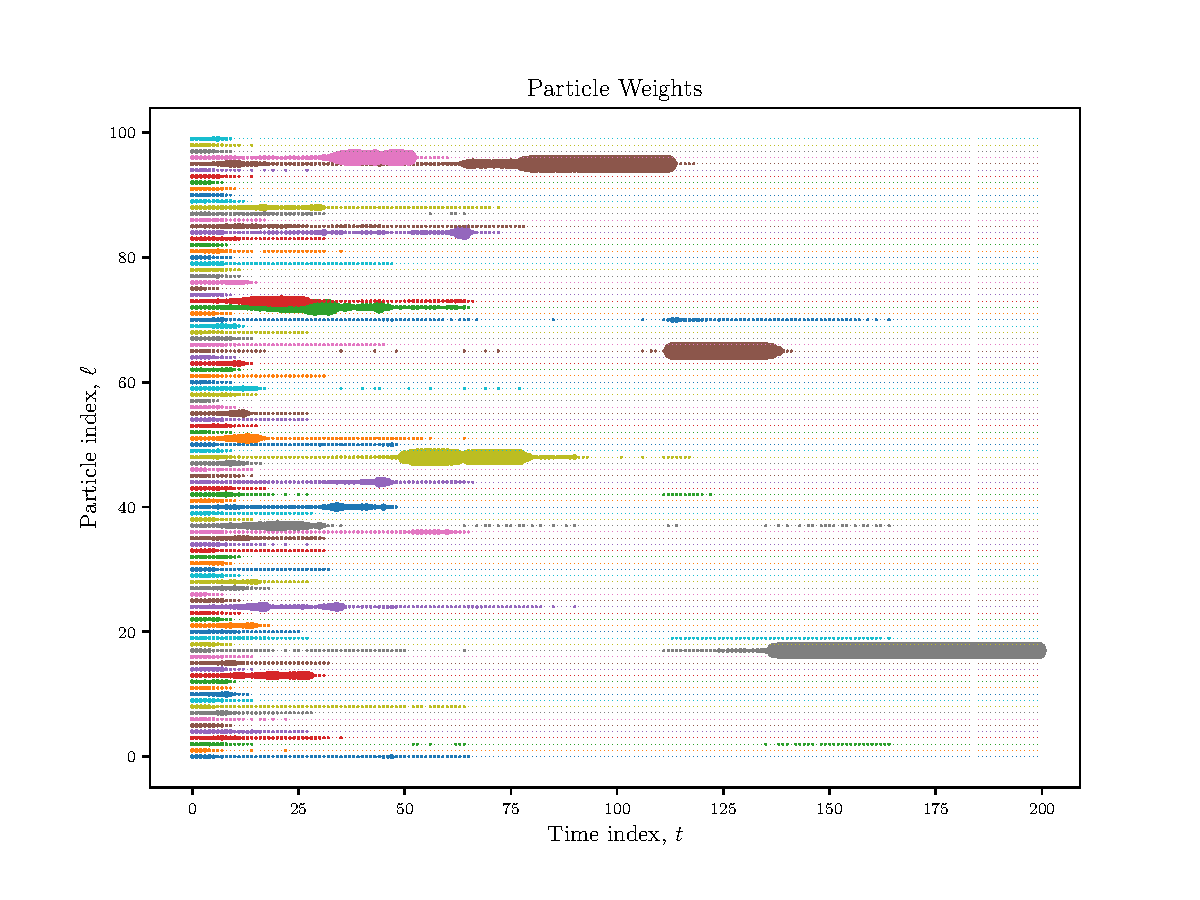
\includegraphics[width=\textwidth]{Figures/particle_weights_sis.pdf}
        \caption{SIS}
        \label{fig:sis-particle-weights}
    \end{subfigure}
    \begin{subfigure}{.5\textwidth}
        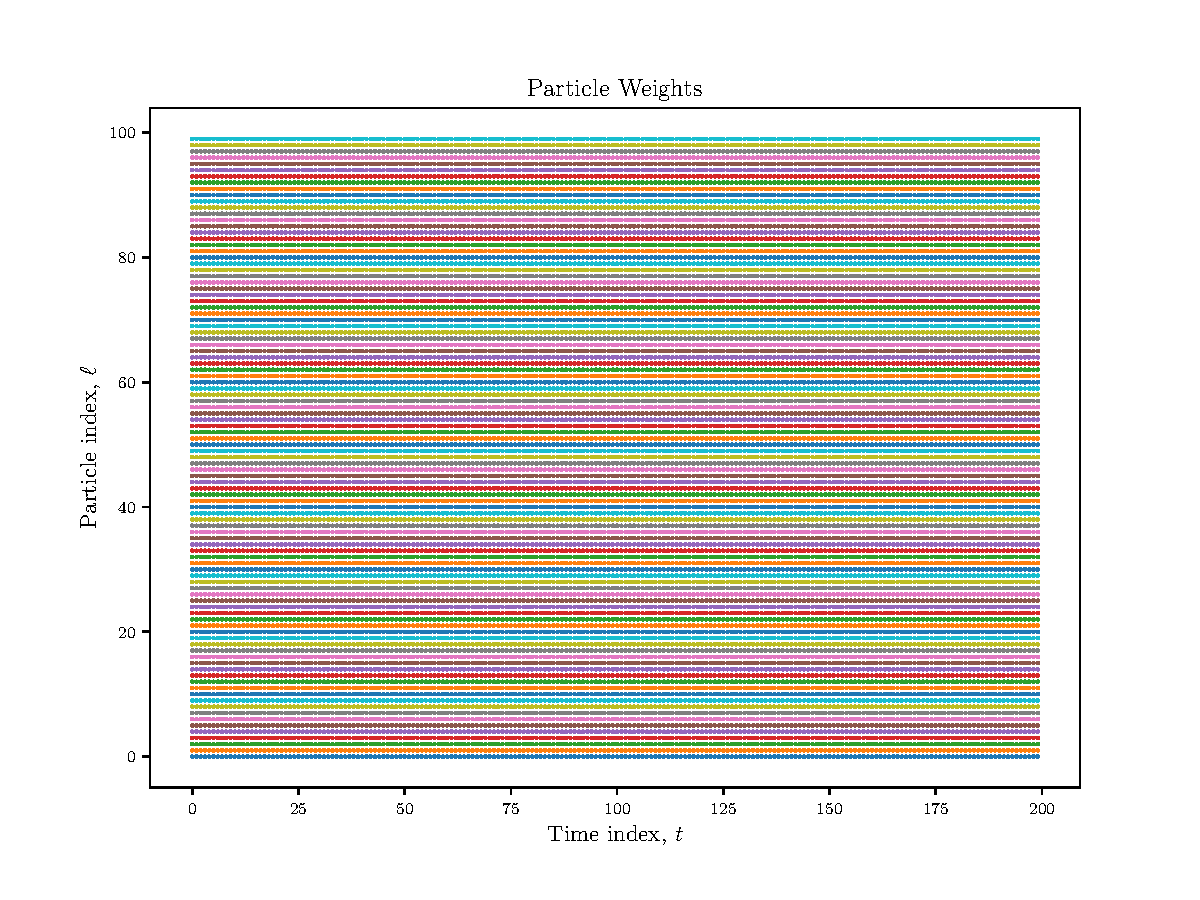
\includegraphics[width=\textwidth]{Figures/particle_weights_sir.pdf}
        \caption{SIR}
        \label{fig:sir-particle-weights}
    \end{subfigure}

    \centering
    \begin{subfigure}{.5\textwidth}
        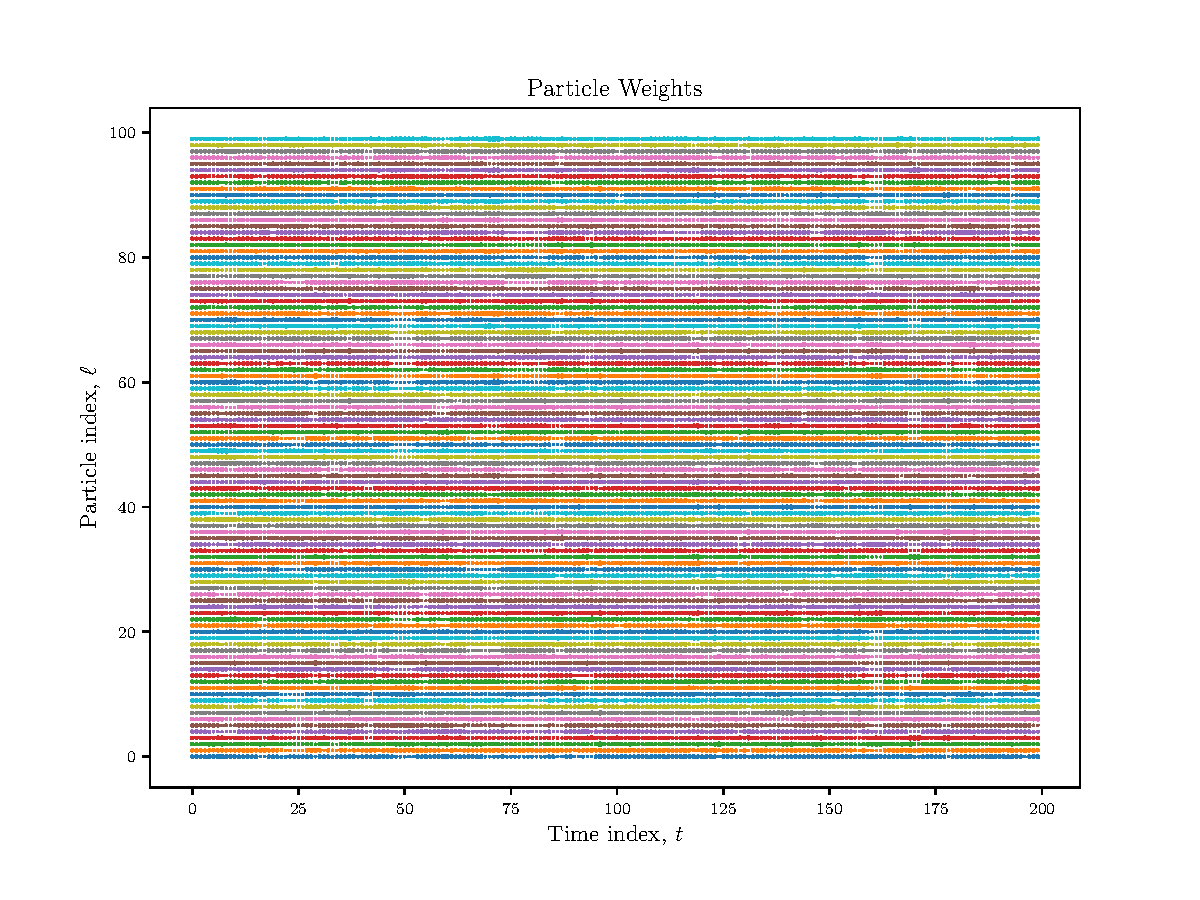
\includegraphics[width=\textwidth]{Figures/particle_weights_sir_thres.pdf}
        \caption{SIR with Threshold}
        \label{fig:sir-thres-particle-weights}
    \end{subfigure}
    \caption{Plot of particle weight size at each time step. The diameter of markers scales with the size of particle weights.}
    \label{fig:particle-weights}
\end{figure}

\begin{figure}
    \centering
    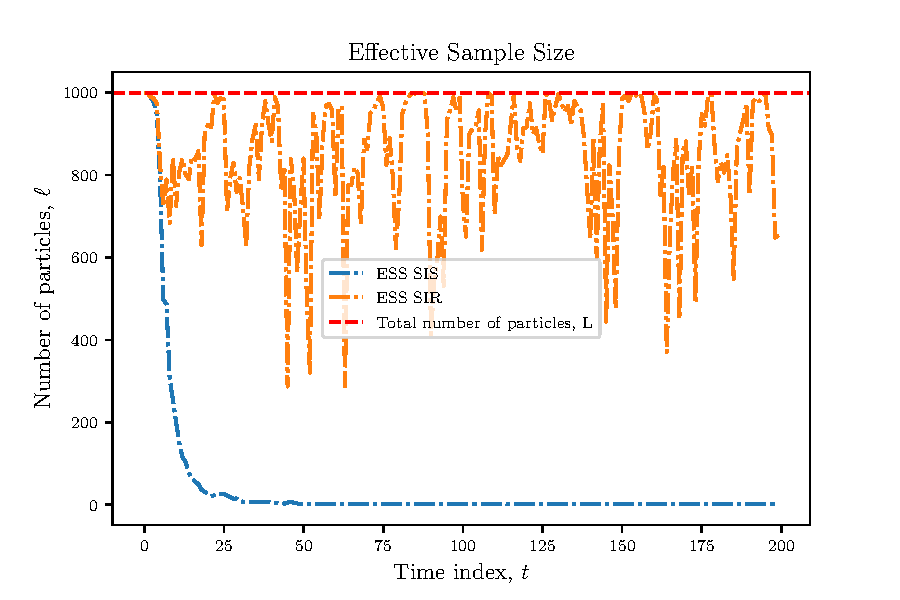
\includegraphics[width=.5\textwidth]{Figures/ess.pdf}
    \caption{Effective sample size of SIS and SIR algorithm.}
    \label{fig:ess}
\end{figure}

\begin{figure}
    \begin{subfigure}{.5\textwidth}
        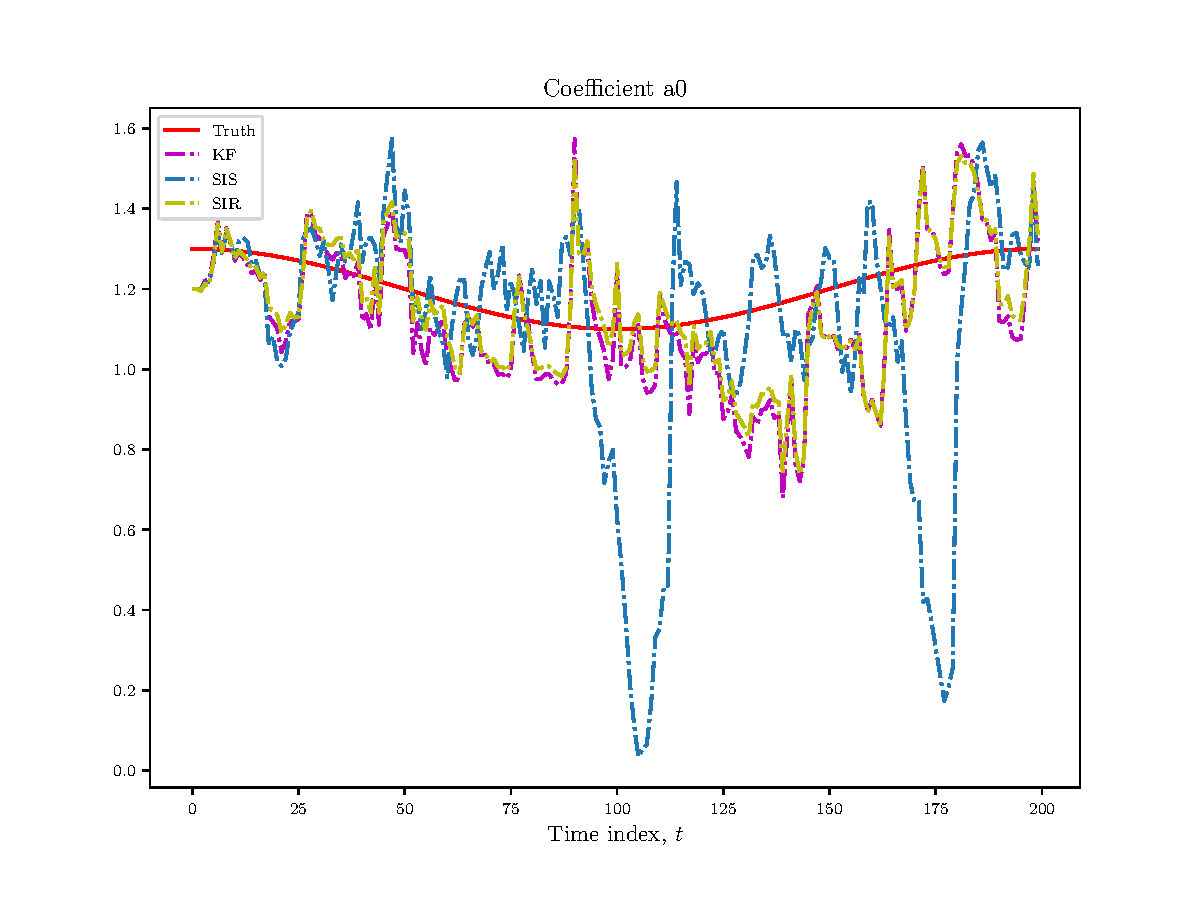
\includegraphics[width=\textwidth]{Figures/coefficient_a0.pdf}
    \end{subfigure}
    \begin{subfigure}{.5\textwidth}
        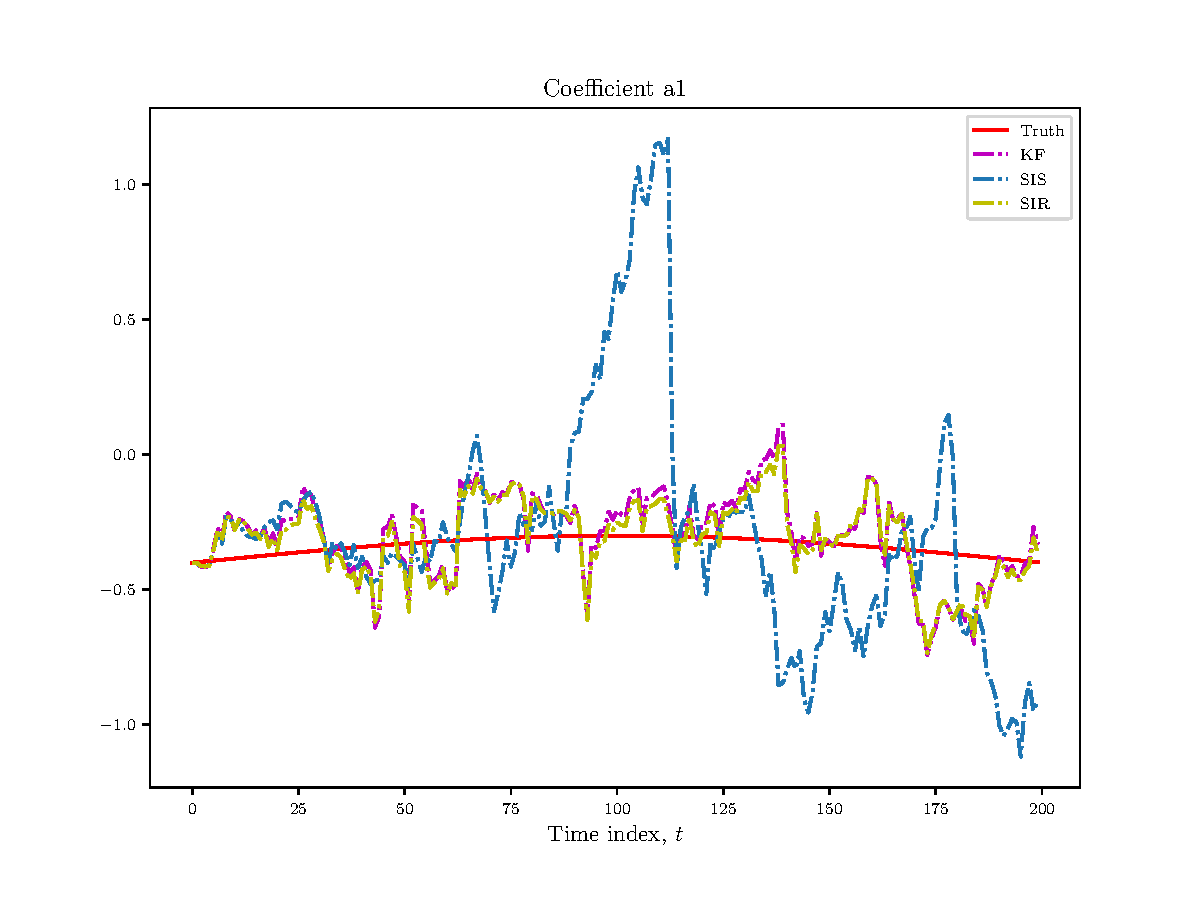
\includegraphics[width=\textwidth]{Figures/coefficient_a1.pdf}
    \end{subfigure}

    \centering
    \begin{subfigure}{.6\textwidth}
        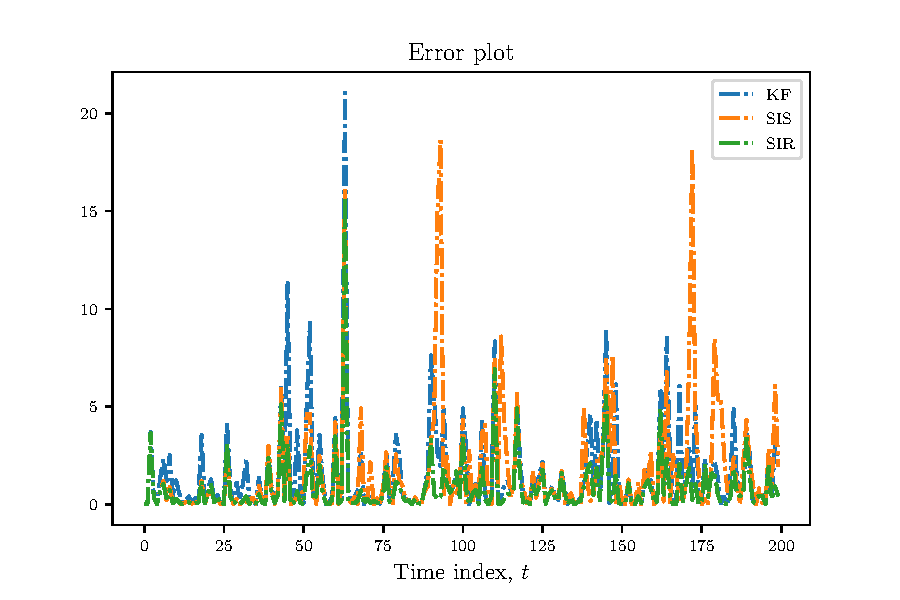
\includegraphics[width=\textwidth]{Figures/error.pdf}
    \end{subfigure}
    \caption{Plots of unknown parameters $a_0$ and $a_1$ estimated using KF, SIS and SIR, along with its squared errors. Mean Squared Error: (KF) 1.2610 (SIS) 1.3363 (SIR) 0.6150 (SIR with Threshold) 0.6071; Average Runtime: (KF, 100 loop average) 0.534s (SIS, 5 loop average) 4.65s (SIR, 5 loop average) 4.68s}
    \label{fig:results-1}
\end{figure}


\section{Task 2} \label{sec:task-2}

Task 2 presents derivations and results of the Extended Kalman Filter (EKF) algorithm for the logistic regression problem described in the Lab 3 exercise sheet. Extended Kalman Filter allows state estimation of non-linear Gaussian state-space models by approximating the non-linear function as its Taylor approximation to the first order. Non-linearity can be present in either or both state and observation models.

Following the exercise sheet, consider we have a simple binary classification problem to be solved sequentially using a logistic regression. We have a state space model:

\begin{equation}
    \begin{split}
        \pmb{\theta} (n) &= \pmb{\theta} (n-1) + \pmb{w}(n)\\
        y(n) &= f(\pmb{\theta}(n), \pmb{x}_n) + v(n),
    \end{split}
    \label{eq:ssm}
\end{equation}

with the non-linear function as the logistic regression:

\begin{equation}
    \begin{split}
        f(\pmb{\theta}(n), \pmb{x}_n) &= g(\pmb{\theta}(n)^T \pmb{x}_n)\\
        g(z) &= \frac{1}{1 + e^{-z}},
    \end{split}
    \label{eq:logistic}
\end{equation}

As mentioned above, \cref{eq:logistic} can be approximated by it's first-order Taylor approximation:

\begin{equation}
    f(\pmb{\theta}(n), \pmb{x}_n) \approx f(\pmb{\theta}(n|n-1), \pmb{x}_n) + \pmb{\hat{F}}_n^T (\pmb{\theta}(n) - \pmb{\theta}(n|n-1))
\end{equation}
    
where the Jacobian is described as:

\begin{equation}
     \pmb{\hat{F}}_n = \pmb{\hat{F}}(\pmb{\theta}(n), \pmb{x}_n) = g(\pmb{\theta}(n|n-1)^T \pmb{x}_n)(1 - g(\pmb{\theta}(n|n-1)^T \pmb{x}_n)) \pmb{x}_n
\end{equation}

With the approximation above, the Extended Kalman Filter equations for the logistic regression problem are:

\begin{equation}
    \begin{split}
        \pmb{\theta}(n|n-1) &= \pmb{\theta}(n-1|n-1)\\
        P(n|n-1) &= P(n-1|n-1) + Q\\
        e(n) &= y(n) - f(\pmb{\theta}(n|n-1), \pmb{x}_n)\\
        \pmb{\theta}(n|n) &= \pmb{\theta}(n|n-1) + \pmb{k}(n)e(n)\\
        P(n|n) &= (I - \pmb{k}(n) \pmb{\hat{F}}_n) P(n|n-1)\\
        \pmb{k}(n) &= \frac{P(n|n-1) \pmb{\hat{F}}_n^T}{R + \pmb{\hat{F}}_n P(n|n-1) \pmb{\hat{F}}_n^T}
    \end{split}
    \label{eq:ekf}
\end{equation}

\cref{eq:ekf} follows the same notation as in \cite{lab3}.

The EKF algorithm described in \cref{eq:ekf} will be utilised to attempt to solve two binary classification problems with different $\alpha$, illustrated in \cref{fig:dataset}. The dataset is generated using Numpy following the instructions in \cite{lab3}.

\begin{figure}
    \centering
    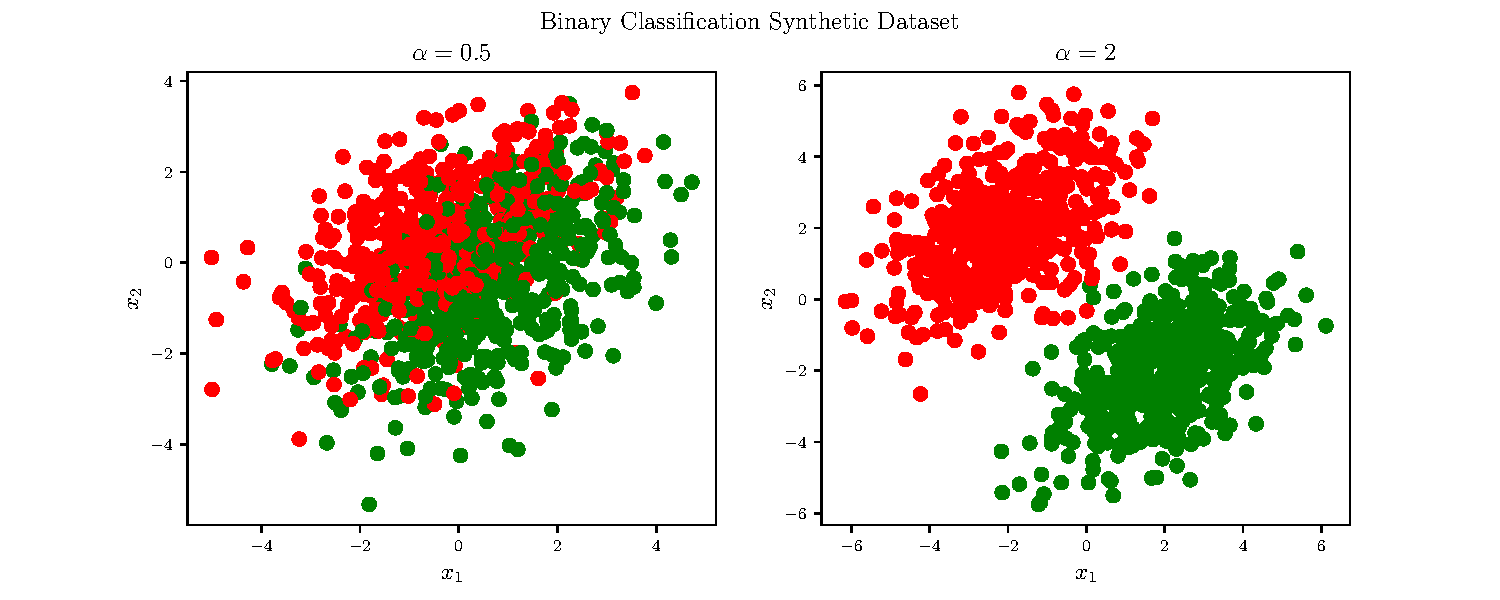
\includegraphics[width=\textwidth]{Figures/dataset.pdf}
    \caption{Binary classification synthetic dataset with different mean $\alpha$.}
    \label{fig:dataset}
\end{figure}

\cref{fig:error_ekf-lr} shows the error plot of both problems. It is shown that an increase in $\alpha$ allows for a better convergence of error. When $\alpha$ decreases, the problem becomes non-linearly separable. Hence, with $\alpha = 0.5$, the convergence of error is not possible with a linear classifier such as logistic regression. The best accuracy is calculated by taking the $\pmb{\theta}$ of the time step of the lowest error.


\begin{figure}
    \begin{subfigure}{.5\textwidth}
            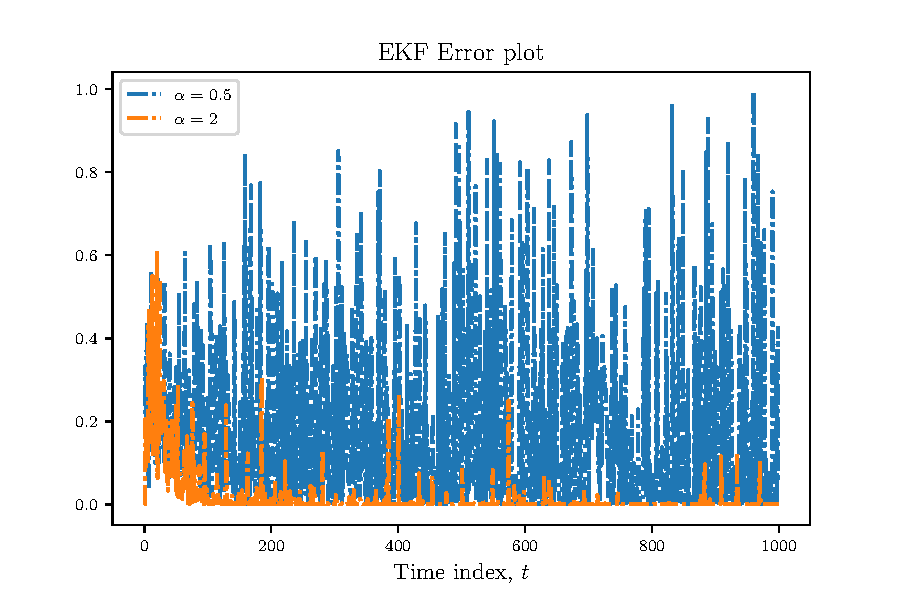
\includegraphics[width=\textwidth]{Figures/error_ekf-lr.pdf} 
            \caption{EKF\\
            Best accuracy: ($\alpha = 0.5$) 76.2\% ($\alpha = 2$) 99.8\%}
            \label{fig:error_ekf-lr}
    \end{subfigure}
    \begin{subfigure}{.5\textwidth}
        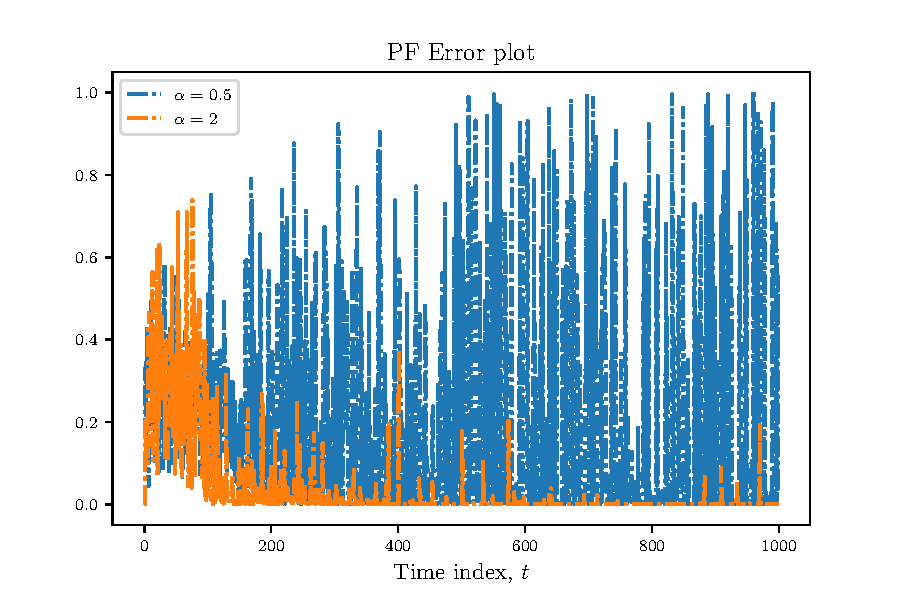
\includegraphics[width=\textwidth]{Figures/error_pf-lr.pdf} 
        \caption{PF; $N_s = 100$\\
        Best accuracy: ($\alpha = 0.5$) 75.6\% ($\alpha = 2$) 99.6\%}
        \label{fig:error_pf-lr}
    \end{subfigure}
    \caption{Logistic regression squared error with different $\alpha$.}
    \label{fig:error-lr}
\end{figure}


\section{Task 3}

Task 3 presents the pseudocode and results of the Particle Filter (PF) algorithm for the logistic regression problem described in \cref{sec:task-2}. In \cref{sec:task-1}, we discussed the superiority of the resampling step when added to the original SIS algorithm. Hence, in this section, the PF algorithm will include the resampling step.

\cref{eq:probabilistic-ssm} shows the probabilistic representation of the state space model described in \cref{eq:ssm}. The assumption is made that both state and observation models are Gaussian. \cref{algo:pf-lr} describes the particle filtering algorithm for the logistic regression problem. \cref{algo:pf-lr} follows the same notation as in \cite{lecture6}.

\begin{equation}
    \begin{split}
        p(\pmb{\theta}(n) | \pmb{\theta}^i (n-1))) &= \mathcal{N} (\pmb{\theta}(n) | \pmb{\theta}(n-1), Q)\\
        p(y(n) | \pmb{\theta}^i(1:n)) &= \mathcal{N} (y(n) | f(\pmb{\theta}(n), \pmb{x}_n), R) 
    \end{split}
    \label{eq:probabilistic-ssm}
\end{equation}


\begin{algorithm}[H]
    \SetKwInput{KwInit}{Initialise}
    \SetKwInput{KwOutput}{Output}              % set the Output
    \SetAlgoLined
    \KwInit{$\{(w^1(0), \pmb{\theta}^1 (0)), \cdots, (w^{N_s}(0), \pmb{\theta}^{N_s} (0))\}$}
    \KwOutput{$\{(w^1(n), \pmb{\theta}^1 (n)), \cdots, (w^{N_s} (n), \pmb{\theta}^{N_s} (n))\}_{n = 1}^N$}
     \For{$n = 1, \cdots, N$}{
        \For{$i = 1, \cdots, N_s$} {
            Sample $\pmb{\theta}^i (n) \sim p(\pmb{\theta}(n) | \pmb{\theta}^i (n-1)))$\; 
            Append $\pmb{\theta}^i (1:n) = (\pmb{\theta}^i (1:n-1), \pmb{\theta}^i (n))$\;
            Evaluate $w^i(n) = w^i(n-1) p(y(n) | \pmb{\theta}^i(1:n))$\;
        }
        \For{$i = 1, \cdots, N_s$} {
            Normalise $w^i(n) = w^i(n) / \sum_{j = 1}^{N_s} w^j(n)$\;
        }
        Resampling\;
     }
     \caption{Particle Filter for Logistic Regression}
     \label{algo:pf-lr}
\end{algorithm}

\cref{fig:error_pf-lr} shows the error plot of the particle filter. Both algorithms show similar results. However, the particle filter has more fluctuations of error. This is due to the small sample size $N_s$ that was used for the algorithm. Increasing $N_s$ will allow less fluctuations at the expense of computation time. The accuracy of classification for both algorithms has proved to be nearly identical.

Note that both EKF and PF are non-optimal filters due to the approximations. However, the advantages of PF is that it is able to work with non-linear non-Gaussian state space models. PF converges to the optimal solution when number of particles $N_s$ approaches infinity. The EKF derivations assumes Gaussianity in the state space model, but is able to solve non-linear problems.


\printbibliography

\end{document}